\chapter{内额皮层:基于输出结果选择动作}

这本书提出了关于灵长类动物前额叶皮层基本功能的方案。
\section{概述}
内侧PF皮层有助于根据这些动作之前的行为结果来评估和选择动作,其连接指纹解释了它是如何做到这一点的。海马连接提供有关导航和其他涉及动作的事件的信息,杏仁核提供基于当前生物需求的预测结果的最新评估,并且与内侧前运动区域的连接提供了行动的途径。这些与行动和动机有关的“内部”信号与感官输入等外部信号形成对比。中间PF区域基于这些内部因素对行动的选择产生偏见,包括努力成本、更新的估值、预测结果对觅食选择的影响,以及使用内在与外在坐标系来指导行动。在灵长类动物中,内侧PF皮层的颗粒部分通过在反馈时间评估自我产生的选择、平衡竞争性任务规则以及根据单个先前事件做出选择来阐述这些“内部”影响。

\section{概述}
内侧PF皮层有助于根据这些动作之前的行为结果来评估和选择动作,其连接指纹解释了它是如何做到这一点的。海马连接提供有关导航和其他涉及动作的事件的信息,杏仁核提供基于当前生物需求的预测结果的最新评估,并且与内侧前运动区域的连接提供了行动的途径。这些与行动和动机有关的“内部”信号与感官输入等外部信号形成对比。中间PF区域基于这些内部因素对行动的选择产生偏见,包括努力成本、更新的估值、预测结果对觅食选择的影响,以及使用内在与外在坐标系来指导行动。在灵长类动物中,内侧PF皮层的颗粒部分通过在反馈时间评估自我产生的选择、平衡竞争性任务规则以及根据单个先前事件做出选择来阐述这些“内部”影响。

\section{介绍}
第一章解释了连接限制了PF皮层的功能。由于其连接因区域而异,本章开始对PF皮层进行区域探索。我们从内侧PF皮层开始,部分原因是它包括PF皮层的一些旧部分(第2章)。\par
第2章区分了内侧PF皮层的颗粒和无颗粒部分,后者在所有哺乳动物中共享。因此,我们想比较大鼠和猴子的无颗粒PF区域。不幸的是,对猴子的这些区域知之甚少。因此,我们被迫依赖啮齿动物(主要是大鼠)的数据。我们认识到这种方法的危险 - 啮齿动物和灵长类动物的最后共同祖先生活在~70-90 Ma,从那以后这两个谱系就分开进化了。这一事实意味着,随着两组动物的进化,两组动物的无颗粒PF区域的连接和功能将发生变化。未来的研究将表明这种差异的程度,但现在我们必须利用我们所拥有的东西来凑合。\par
在灵长类动物中,内侧PF皮层位于内侧前运动区域的喙部,包括前SMA,SMA和CMA(见缩写列表)。帕辛汉姆等(2010)认为,所有这些中间领域都显示出指导和分析基于“内部”信号的行动的专业化。“内部”一词,在这里使用的意义上,是指传达内部状态和记忆的信号,与视觉、听觉、嗅觉、味觉和触觉等外部信号形成鲜明对比。

\section{区域}
图3.1显示了猴子和人类中被指定为内侧PF皮层的区域,图2.1显示了其在猴子,人类和大鼠中的细分视图。在灵长类动物中,内侧PF皮层的颗粒部分由前扣带皮层(区域24),边缘前皮层(主要是区域32)和边缘下皮层(区域25)组成。正如第2章所解释的,所有哺乳动物,包括啮齿动物和灵长类动物,都有这三个区域的同系物。\par
内侧PF皮层的颗粒部分包括区域9的内侧部分和所有区域10,只有灵长类动物有这些区域。第1章证明将极地包括在内是合理的PF皮层(区域10)在内侧区域组,部分基于连接。注意我们将所有极性PF皮层(区域10)都包括在周一的内侧PF皮层内键,但只是它在人类中的内侧部分。
\begin{figure}[!htb]
	\centering
	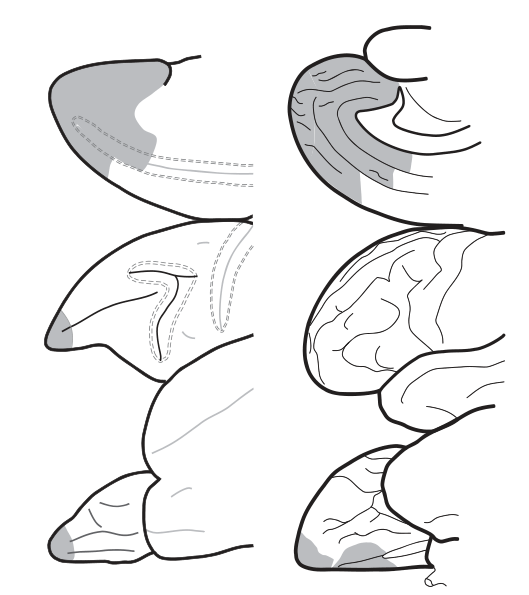
\includegraphics{image_pfc/Fig_3_1}
	\caption*{图3.1 猕猴(左)和人类(右)的内侧PF皮层,用阴影表示。格式如图1.2所示。}
\end{figure}

术语前扣带皮层在文献中有很多含义。在这本书中,我们将边缘前皮层和边缘下皮层排除在我们称为前扣带皮层(图2.1)。我们还排除了扣带运动区域,这些区域我们认为是前运动皮层的一部分。因此,读者应该意识到当我们使用短语 前扣带皮层 ,我们仅指区域 24 的一部分,而不是到运动前区域或内侧PF皮层的其他颗粒状部分。\par
在我们排除在前扣带皮层之外的区域中,眶前和边缘下皮层占据了大部分的眶前和眶下皮层。术语膝下皮层是指胼胝体膝腹侧的皮层,术语膝前皮层是指位于膝侧的无核区域。孕皮质不包括位于更前列的颗粒区域,例如极性PF皮质的内侧部分(区域10)。最后,我们称之为腹内侧PF皮层的14区的状态仍不确定。一些专家将其纳入内侧PF皮层,另一些专家则将其视为眼眶PF皮层的最内侧部分。我们不需要在这些分类之间做出决定,但在大多数情况下,我们保留了第4章关于眼眶PF皮层的区域14的考虑。\par

\section{关系}
图3.2显示了猕猴内侧PF皮层的主要连接。
这个情节和第4-7章中的类似情节旨在传达神经解剖学文献中出现的最重要的概念点。我们不打算提供一个全面的总结,也不关心指出哪些神经解剖学家首先描述了一个特定的途径。这些情节起到了连接指纹的作用,第一章对此进行了解释。连接指纹强调区分PF皮层区域彼此和其他皮层区域的特征,就像人类指纹区分人与人一样。\par
1.海马体和下托与内侧PF皮层的边缘下和边缘前区域有密集的相互连接(Insausti和Muñoz 2001)。海马体和内侧PF皮层之间的间接连接包括前扣带皮层(区域24)和内侧颗粒区域9和10,其中一些通过脾后皮层运行(Kobayashi和Amaral 2003)。内嗅皮层和海马旁皮层也与内侧PF皮层有联系(Kondo等人)\par
2.2003 ; Muñoz和Insausti(2005年)。海马体和内侧PF皮层之间的皮质下通路包括通过乳头体和丘脑的中继。我们认为与海马体的联系对内侧PF皮层的功能特别重要。其他PF区域,如外侧OFC,要么缺乏与海马体的连接,要么具有非常弱的连接(Carmichael和Price 1995a)。稍后,我们解释了我们的观点,即海马体为PF皮层提供了有关导航和其他涉及动作的过去事件的信息。2.内侧PF皮层与杏仁核有着紧密的联系,图3.3显示,这些投射中密度最大的涉及PF皮层的无核部分\par
\begin{figure}[!htb]
	\centering
	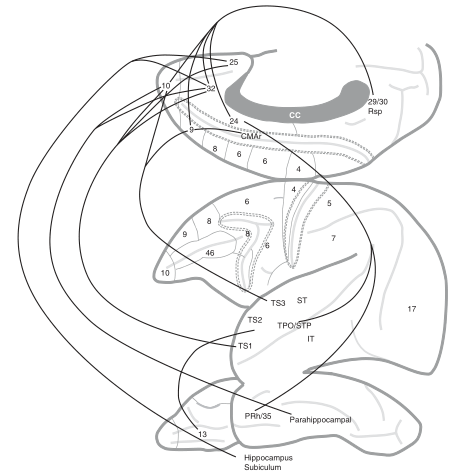
\includegraphics{image_pfc/Fig_3_2}
	\caption*{图3.2猕猴内侧PF皮层的选定连接。图1.4和1.5给出了沟和区域的名称。线连接着一些有直接轴突连接的区域,除非另有说明,否则假设是相互的。}
\end{figure}
(Prather等人,2001年;Morecraft等人,2007年)。颗粒区域,如13m区域,也接受杏仁核输入,图3.3没有说明(Saleem等人,2008年)\par
杏仁核通常被视为在情绪、动机和奖励中发挥作用,包括恐惧调节和对社会刺激(如人脸)的情绪反应。但它在奖励中的作用并不是一般的。双侧杏仁核损伤后,条件性视运动学习完全正常进行,尽管这取决于学习与奖励的关系(Murray和Wise 1996)。因此,奖赏处理本身不能作为杏仁核功能的一般或完整描述。相反,最有力的证据表明,杏仁核和皮层之间的相互作用会根据当前的需求更新结果评估(Baxter和Murray,2002年)。在整本书中,我们使用结果一词来指代以下反馈\par
\begin{figure}[!htb]
	\centering
	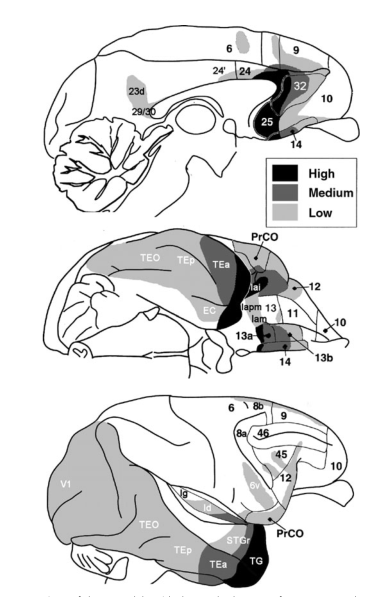
\includegraphics{image_pfc/Fig_3_3}
	\caption*{图3.3猕猴杏仁核与大脑皮层的连接。阴影表示投射的主观密度,重点是从杏仁核到皮层的投射。皮层通常也会发送一个返回投影。缩写:EC,内嗅皮层;Iai、Iapm和Iam,分别为无核岛状区、下分区、后内侧分区和内侧分区;Ig,颗粒状岛叶皮层;Id,粒状岛叶皮层;中央前顶盖皮质;颞上回;TEa、TEp、TEO、颞下区、前部、后部和枕部;TG,颞极皮层;V1,初级视觉(纹状体)皮层(17区)。经麦克米伦出版有限公司(Macmillan Publishers Ltd.)普莱斯·JL(Price JL)、德雷维茨·WC(Drevets WC)许可转载。《情绪障碍的神经回路》,《神经精神药理学》35:192–216,©2009,自然出版集团}
\end{figure}
一种行动,无论是从发生的事情还是在任何特定时间的价值来看。当然,目前的需求不仅涉及营养和液体,还涉及避免伤害和其他生物成本和收益。因此,我们可以说杏仁核有助于评估积极和消极的结果。\par
3.内侧PF皮层直接或间接投射到运动前区域。颗粒内侧PF皮层(9区)与内侧PF皮层的其他部分有联系,特别是与前扣带皮层有联系(Vogt和Pandya 1987)。该区域反过来与前扣带运动区(CMAr)相连,CMAr是内侧前运动皮层的一部分(Morecraft和Van Hoesen,1998)。CMAr位于扣带沟(Dum和Strick,2002年),位于与之相连的术前运动区(preSMA)的腹侧(Luppino等人,1993年)。SMA本身也与尾扣带运动区相互连接(Luppino等人,1993年)。扣带运动区或前SMA和SMA的损伤损害了猴子在没有外部(感觉)提示的情况下做出的运动的产生(Thaler等人,1995年)。因此,我们可以将这些行动称为“内部”指导\par
4.与腹侧PF皮层和眶侧PF皮层不同,内侧PF皮层不接收来自颞下皮层的视觉输入(Carmichael和Price 1995b;Kondo等人2005)。然而,前扣带皮层与嗅周皮层有一些联系,它也接收来自颞上沟TPO区域的输入(Kondo等人,2005年),该区域处理视觉和听觉信息。尽管有这些输入,内侧PF皮层和视觉区域之间的联系并不是特别突出。\par
5.内侧PF皮层,尤其是极性PF皮层(区域10),接收来自颞上皮层的投射,其中大部分来自其吻部,包括颞极(Barbas等人1999;Kondo等人2003)\par
这些投射中一些更尾部的涉及生理学研究表明是听觉的区域(Hackett et al 1998),但其他投射的功能,如靠近颞极的投射,仍然未知\par
6.与PF皮层的许多其他部分不同,内侧PF皮层也投射到下丘脑(Rempel-Clower和Barbas,1998年),以及在内脏运动功能中发挥作用的脑干网状核(Öngür等人,1998年;Barbas等人,2003年)\par
其中一些投射可能会影响自主神经系统,以及大脑控制身体的其他方式。例如,下丘脑外侧调节自主神经的唤醒,下丘脑的室旁核控制神经内分泌和神经分泌的输出。\par
\subsection{总结}
内侧PF皮层的连接指纹表明以下要点:(1)与PF皮层的其他部分相比,内侧PF皮层接收的感觉输入很少;(2) 它与运动前区域相连,该运动前区域在动物蓄能器网络71缺乏来自任何外部线索的动作提示时控制动作;(3)它与海马体和杏仁核有着密切的联系,这表明它既可以获得过去事件的记忆,也可以获得从当前生物需求来看有价值的结果信息\par
尽管这里列出的连接并不总是涉及内侧PF皮层的相同部分,但不同部分相互连接(Barbas 2000),这意味着一个部分的输入可以影响其他部分。第8章将这一观点扩展到整个PF皮层。\par
\section{决策、选择和目标}
尽管“决定”一词可以应用于动物所做的大多数事情,但我们使用这个词的方式更为有限。我们将决策与这些决策之后可能做出的选择和采取的行动区分开来(Schall 2001)。决策涉及基于感官输入的感知。从这个意义上说,决定并不是直接指动物所做的任何事情。
因此,动物会做出感性的决定,而不是感性的选择。它们做出觅食的选择,而不是觅食的决定\par
作为其决策的结果,动物可能会选择一个目标,并基于这个目标的选择,它可能会选择行动。或者,动物可以直接在动作中进行选择。在整本书中,我们使用目标一词来指代动物选择作为其行动目标的物体或位置。然后,这一行动产生了一个结果,包括动物所获得的利益或因其行为而产生的成本。因此,我们将目标与结果区分开来,从不将目标一词用作结果的同义词。\par
我们知道,在文献中,使用目标一词来表示动物在行为实验中获得的奖励是很常见的。事实上,在这些实验中,奖励是动物的最终目标。但为了获得奖励,动物通常必须选择一个物体或地点作为其行动的目标。因此,我们为这些对象和地点保留目标,并始终使用结果来奖励和其他形式的行动或事件反馈。这个术语有助于本书中许多地方的讨论,读者需要记住我们使用这些术语的方式,以及它与文献中其他使用的不同之处\par
我们还区分了基于外部或“内部”线索的选择(Passingham等人,2010年)。例如,猴子可以使用远处的视觉标志来选择觅食目标,比如远处树上的水果或树叶。因此,它们根据外部的感官信号产生一个目标——水果或树叶。但猴子也可以根据它们的记忆或内部状态的变化(如饥饿)来产生目标。由于没有更好的词,我们说在这种情况下,动物是根据“内部”信号行事的。稍后,我们将讨论内侧PF皮层在外部和“内部”信号竞争时的作用\par
\section{累加器网络}
累加器-赛道模型为这种神经竞争提供了一种机制,因此我们在这里给出了一个非常简短的描述。尽管累加器网络已经了解这些模型将使读者更容易理解对内侧PF皮层的输入如何导致动作,以及来自内侧PF皮质的输出如何会使其他类似网络产生偏见。在本章的后面,我们将看到这些想法在内侧PF皮层的功能中的具体应用,这些功能可以做出与觅食类似的选择\par
猴子的神经生理学实验说明了累加器网络是如何工作的。当神经网络达到产生输出的阈值时,就会做出决策、选择和行动。这些网络就像漏洞百出的积分器,积累有利于其输出的“证据”:网络所代表的决策、选择或行动。一旦它们达到阈值,网络的输出就会引起一系列影响,这些影响可能最终导致电机命令的执行,要么通过驱动电机模式发生器的活动,要么将其从紧张抑制中释放出来。各种类型的累加器网络并行运行,因此可以说是相互竞争\par
图3.4显示了一个弹出实验的结果。在这类实验中,猴子的视野中会出现许多刺激物。它们大多数都有相同的特征,如颜色和形状,但有一个不同。在得出图3.4的实验中,猴子看到了七个红色方块和一个绿色方块,这八个刺激物在以注视点为中心的圆的圆周上等距出现。为了在每次试验中获得奖励,猴子必须做一个扫视的眼球运动来固定绿色的正方形。与所有任务一样,从八种刺激出现到猴子开始运动的时间(称为反应时间)因试验而异,但通常在175-225毫秒之间。在第5章中,这个实验涉及眼球运动这一事实变得很重要,但就目前而言,运动的种类无关紧要。\par
\begin{figure}[!htb]
	\centering
	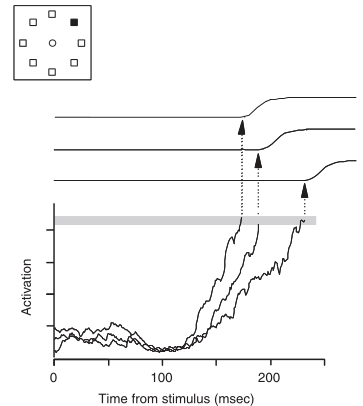
\includegraphics{image_pfc/Fig_3_4}
	\caption*{图3.4额视野中的神经元活动。放电速率是刺激开始后时间的函数。随着活动的增加,它达到了扫视眼球运动的阈值(阴影水平条)。试验根据反应延迟分为三部分。左上角的插图显示了猴子观察到的显示,其中一个刺激因其不同的颜色(黑色方块)而从八个刺激中“弹出”。转载自Schall JD,Thompson KG。视觉引导眼球运动的神经选择和控制。神经科学年度评论22:241–59©1999年年度评论,以经许可}
\end{figure}
累加器模型假设一些累加器集成了绿色刺激的证据。可以说,这些累加器体现了一个“假设”,即刺激是绿色的,其输入是支持和反对这一假设的证据。在单细胞水平上,信息的积累表现为上升的活动,直到达到阈值,有时称为爬升活动。图3.4显示了这种攀爬活动,分为三组试验,根据猴子的反应时间进行排序。在最短的反应时间内,细胞上升到由水平灰色条指定的给定水平,然后扫视很快开始。没有直接证据表明这类神经元的整个网络在那一刻达到了阈值,但我们认为是这样。如图所示,活性增加的速率越慢,反应时间越长\par
竞争的产生是因为这些神经网络的架构及其相互作用。首先达到阈值的网络“赢得”比赛,它控制着它所代表的决策、选择或行动。总的来说,这些回路以赢者通吃的方式工作,这反映了一个事实,即动物不能同时移动两个相反的方向,同样,在大多数情况下,也不会同时做出相互矛盾的决定和选择。\par
猴子必须辨别相干运动方向的实验说明了累加器网络的竞争方式。在这项任务中,许多光点以相同的速度向同一方向移动,而其他光点则随机移动。随着观看时间的延长和更多的光点向同一方向移动,决策的准确性会提高。Gold和Shadlen(2007)已经回顾了这些神经元机制的证据。根据他们的分析,几个区域的细胞增加了它们的活动,直到它们达到阈值:MT和MST区域的网络代表决策,LIP区域的网络表示选择,而FEF区域的网络则代表行动(Kim和Shadlen,1999)。\par
图3.5显示了自上而下的有偏见的竞争是如何运作的。在这种情况下,实验者在MT区域使用皮质内微刺激来模拟自上而下的信号。以一个整合了向上运动证据的网络为例。通过刺激网络中的神经元,它比没有微刺激的情况下更快地达到阈值。这种人为的输入使“向上”的累加器更有可能赢得“比赛”,并做出圆点向上移动的决定。\par
活动上升到网络阈值,从而产生决策、选择或行动的速度取决于证据的强度和整合证据的可用时间。它还取决于竞争累加器的活动,这些累加器为替代决策、选择和行动收集证据。\par
\begin{figure}[!htb]
	\centering
	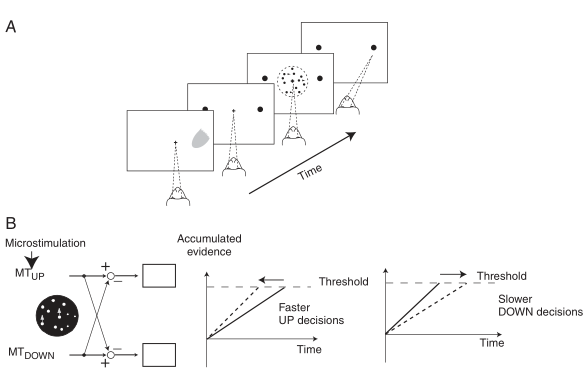
\includegraphics{image_pfc/Fig_3_5}
	\caption*{图3.5自上而下注意力的神经机制。(A) 猴子观察斑点,并在左右扫视目标之间进行选择,以报告斑点运动的方向。虚线在固定点处汇合。(B) 一些累加器网络集成了点向上移动的证据,另一些则集成了点向下移动的证据。当点向上移动时,由于皮质内微刺激,网络中的更大活动会导致其更快地达到“向上”决策的阈值,而“向下”决策的速度较慢(虚线)。缩写:MT UP,位于颞中区的细胞编码向上的斑点运动;MT DOWN,编码向下运动的细胞。+,兴奋性突触输入,抑制性输入。虚线显示皮质内微刺激期间的活动率;实线显示了在这种刺激之前和之后的活动。(A) 复制自Roitman JD,Shadlen MN。在组合视觉辨别反应时间任务中,顶内外侧区域神经元的反应。《神经科学杂志》22:9475–89©神经科学学会,2002年,经许可。(B) 转载自Ditterich J,Mazurek ME,Shadlen MN。视觉皮层的微刺激会影响感知决策的速度。《自然神经科学》6:891-8©2003。}
\end{figure}
作为“种族”的一个重要方面,积累矛盾证据的细胞可以相互抑制,如图3.5所示。其他因素也会影响每个“种族”,包括每个网络的阈值、其兴奋性水平,以及推翻或否决决定、选择或行动的信号。总之,这些网络中的许多网络之间的相互作用允许层次更高的网络对低阶网络产生的结果产生偏见。对于内侧PF皮层,这涉及到与海马体、杏仁核、运动前皮层、下丘脑、中脑导水管周围灰质和其他结构的相互作用\par
在后面的章节中,我们认为PF皮层的其他区域也会对低阶区域发生的竞争产生偏见。例如,第5章提供的证据表明,尾部PF皮层可以对视觉区域施加自上而下的偏见,以增强对运动或形状的处理,这取决于它们与手头任务的相关性。同样地第8章认为,当任务需要对行为进行集中控制时,PF皮层作为一个整体会产生自上而下的影响。\par
\subsection{总结}
像单电池一样,累加器网络集成输入,当它们达到阈值时,就会产生输出。这些模型在证据和表征方面为决策、选择和行动提供了一种看似合理的神经元机制,而不仅仅是“祖母细胞”概念所体现的输入和发射。\par
为了总结本章的内容,内侧PF皮层有一组独特的连接,其特征是缺乏感觉输入,与海马体、杏仁核和内侧前运动皮层的相互作用密切。其中一些连接驱动内侧PF皮层中的网络,一些连接将内侧PF皮层的输出传递到大脑的其他部分,在那里它们提供自上而下的偏置。在下一节中,我们提出了一些证据,证明内侧PF皮层的无核部分偏向于竞争控制行为的低阶系统之间的竞争。\par
\section{啮齿类动物的无核皮层}
Murray等人(2011)提出,通过偏置争夺控制行为的大脑系统之间的竞争,内侧PF皮层可以在不直接产生运动命令的情况下影响动物的动作。这个想法解释了哺乳动物的祖先在没有内侧PF皮层的情况下是如何相处得如此融洽的。在没有这些领域的情况下,相互竞争的系统之间的联系最强。这种力量平衡可以改变,但只能慢慢改变。当它在早期哺乳动物中进化时,无核PF皮层提供了一种自上而下的偏见,促进了更快的变化,而不是一种全新的变化能力。后来,特别是在第8章和第9章中,我们提出这种进步——更快的变化,更少的错误——在PF皮层的进化过程中反复发生,第5章对自上而下的偏见竞争进行了更一般的处理。\par
脊椎动物的许多行为都依赖于系统发育上古老的强化学习机制。其中包括古典(巴甫洛夫)和工具(操作)条件反射(Dickinson 1980)。在传统的动物学习理论中,奖励会加强存在时活跃的联想,这一过程被称为强化。
通过这种强化学习机制,刺激、反应和结果的表征之间会产生关联。每个表示可以链接到其他表示,并且它们可以分别缩写为S、R和O。在经典条件反射中,刺激S与结果O相关联,可以称之为S–O映射。在仪器条件作用中,反应R与结果O相关联,称为R–O映射。在后一种情况下,这种关联可能发生在特定的刺激上下文S中,从而产生S–R–O映射。“反应”和“行动”这两个术语的含义差别不大。前者通常意味着存在一种启动刺激,而后者则不需要。我们不时方便地使用S–R、R–O等的紧凑表示法,而不区分动作和响应\par
在动物获得了特定的S–R–O和R–O关联的丰富经验后,它们的行为失去了对结果的依赖,并成为一种习惯。程序性记忆一词有时用来指习惯,与陈述性记忆形成对比。我们避免使用这些术语,因为陈述性记忆的概念通常意味着意识,而我们不能谈论非人类动物的类人意识。\par
Balleine等人(2003)使用了一个简单的程序来区分结果导向的动作和习惯动作。实验人员可以操作性地调节动物执行给定的动作,从而产生一种奖励结果。他们还可以让同一只动物进行第二次动作,从而产生第二种奖励结果。一般来说,受试者发现这两种奖励都是可取的,尽管他们通常有偏好。接下来,受试者有机会消费两种奖励中的一种,通常是饱腹感。消费这种奖励会使其相对于其他选择贬值。在以后的测试中,被称为测试阶段,受试者可以在这两个动作之间做出选择。除非他们养成了某种习惯,否则受试者将把大部分时间花在工作上,以获得最有价值的回报,这是根据他们当前的需求来评估的。这意味着他们会避免产生最近消耗的奖励的行为。因此,对其中一个奖励的讽刺会影响他们的行动选择。\par
大多数心理学家将这种性质的行为称为目标导向行为。但正如我们已经提到的,我们保留目标一词来指行动的目标。因此,我们将这些行为称为结果导向行为。\par
这些实验的一个重要特征是,动物在测试阶段接受任何奖励结果之前选择自己的行动。也就是说,他们不需要在目前的饱腹状态下体验贬值的食物。相反,受试者预测他们的行为将产生的奖励的价值,并据此做出选择。\par
在动物在这类任务上获得了如此多的经验,以至于养成了习惯之后,对其中一种奖励的满足感就不再影响它的行动。动物继续选择在最近的一段时间内导致特定结果的行为,通常是首选食物,尽管这种结果已经贬值。习惯也被称为S–R关联,因为动物在没有参考预测结果的情况下选择行动。养成一个习惯所需的训练量被称为过度训练。\par
请注意,一些专家以一种不那么严格的方式使用“习惯”一词,指的是动物经常做的或人们可以不去想就做的任何事情。
所以读者需要知道,我们不会以这种膨胀的方式使用习惯。\par
早些时候,我们解释了蓄能器-赛道模型的基本原理。现在我们可以将这些原则应用于过度训练动物的习惯生成。根据累加器-赛道模型,一旦S–R关联变得足够强大,以至于它们的累加器网络总是在任何竞争网络达到它们的阈值之前达到阈值,习惯就会盛行。例如,假设S–R网络与S–R–O网络竞争。我们假设,随着S–R网络中连接的加强,它们将更快地达到阈值。当这个过程达到没有其他网络可能“赢得”比赛的地步时,一种习惯就形成了。当一种联想支配着其他人,这可以被称为前置,而前置行为、前置反应和前置行动都指的是这一观点。这些术语既适用于天生的行为,也适用于那些由丰富经验灌输的行为。预备行为在相对稳定的环境中提供了优势。\par
然而,对荒谬行为的依赖有代价也有好处。它们的缺点是动物只能相对缓慢地适应新的条件。在一个经典的例子中,绿色蜥蜴(Lacerta)天生倾向于接近绿色,因为绿色会引导它们走向树叶,从而提供伪装和捕捉猎物的机会。Wagner(1932)试图教这些蜥蜴在与理想食物相关的红色刺激和与掺假食物相关的绿色刺激之间做出选择。训练蜥蜴选择红色刺激需要数百次试验,有些蜥蜴无法做到,尽管它们很容易区分红色和绿色。蜥蜴的优越行为在它们通常的生态位中表现良好,但因此它们无法灵活适应动荡的环境。\par
然而哺乳动物可以相对较快地学会这项任务。Murray等人(2011)提供了非哺乳动物脊椎动物行为不灵活的其他例子,与哺乳动物的灵活性形成对比。例如,老鼠可以学习位置任务的匹配。
在这项任务中,老鼠必须学会回到它们刚刚得到食物的地方(Marighetto等人,1998年)。为了成功地完成这项任务,老鼠必须克服一种天生的倾向,即探索它们最近没有利用过的觅食地点,并避开那些它们已经利用过的地点。完整的大鼠可以在15-20次训练中学习这项任务,但在内侧PF皮层的边缘前和边缘下区域受损后,大鼠的学习速度要慢得多(Dias和Aggleton 2000)。因此,与缺乏这些区域的动物相比,内侧PF皮层似乎赋予了更快、更少错误地从优势行为转变的能力。\par
另一项观察结果强化了这样一种观点,即病变大鼠无法轻易克服其天生的倾向:同样的病变大鼠可以以大约正常的速度学习不匹配定位任务(Dias和Aggleton 2000)。在这项任务中,动物必须避开刚收到食物的地方,选择迷宫的另一个分支。因此,老鼠不必克服它们避开最近被开发的觅食地点的优越倾向。这些想法解释了为什么患有边缘前和边缘下皮层病变的大鼠可以以正常的速度学习非匹配定位任务,但以异常缓慢的速度学习高度相似的匹配定位任务。\par
在野外,不同觅食地点的趋势在许多情况下都提供了优势。耗尽的食物来源几乎没有什么好处。然而,在某些情况下,例如当资源异常迅速地补充时,优势在于动物能够了解这种更新可能发生的背景,并能够抑制在其他地方寻找食物的优越倾向。通过这种方式,皮层下大脑系统的上下偏置可以增强觅食选择的灵活性,而内侧PF皮层似乎在哺乳动物中提供了这种能力。表3.1列出了动物在选择动作时面临的一些问题,以及内侧PF皮层可能带来的一些优势。\par

表3.1选择行动的基本问题\par
\begin{tabular}{c c }	 % 双竖线
	\hline	% 表格横线
	问题 & 解决方案 \\	
	\hline  % 横线
	不同的行动在回报和努力方面产生不同的结果 & 基于习得动作-结果关联的偏倚觅食选择 \\
	\hline
	动作可以基于外在坐标也可以基于内在坐标 & 偏向于那些基于外在或内在规则的觅食选择 \\
	\hline
	动作可以发生在稳定或易失的环境中 & 分别偏向那些基于习惯或基于预测结果的觅食选择 \\
	\hline
\end{tabular}

\section{吸收前皮层和结果导向行为}
在大鼠中,内侧PF皮层包括三个区域,即前扣带皮层、边缘前皮层和边缘下皮层(见图2.1)。正如我们已经提到的,位置匹配和不匹配任务的结果有助于阐明边缘前皮层的作用,但不能区分它们。然而,有几项研究试图这样做。\par
当结果值发生变化时,脊髓前皮质的损伤会损害大鼠改变其行为的能力。上一节描述的贬值测试揭示了动物根据当前需求调整选择的能力。大脑皮质前病变的大鼠继续做出反应,产生高度贬值的奖励。因此,前大脑皮层的损伤导致习惯性行为占主导地位,而非外向性行为(Balleine和Dickinson 1998;Corbit和Balleine 2003)。因此,我们可以得出结论,在正常大鼠中,前大脑皮层会根据结果导向的行为而不是习惯产生对觅食选择的偏见。\par
学习后发生的吸收前皮层损伤没有这种影响(Ostlund和Balleine 2005),这也与该区域产生对结果导向行为的偏见的观点一致。S–R联想(习惯)与S–R–O联想同时发展。经过广泛的经验,习惯可以控制行为,因此前大脑皮层的影响变得不那么重要了。\par
边缘下皮质似乎提供了相反的偏见。Killcross和Coutureau(2003)发现,边缘前皮质和边缘下皮质的作用存在双重分离。他们证实了刚刚提到的这一发现,即大脑前皮层的损伤使大鼠对实验操作的当前奖励值不敏感。边缘下皮质的病变没有这种影响。在这些损伤之后,即使经过了通常会产生习惯性行为的漫长过度训练期,大鼠的选择仍然会受到当前奖励值的影响。因此,我们可以得出结论,在正常大鼠中,边缘下皮层提供了对习惯的偏见。如果没有这种偏见,即使在预期习惯的情况下,行为仍然是以结果为导向的。\par
这些发现表明了这些区域在正常大鼠中所起的作用:边缘前皮层基于S–R–O关联(结果导向的行为)使行为偏向于觅食选择,而边缘下皮层则对同时发生的行为产生偏见学会了S–R联想(习惯)。更广泛地说,这些领域似乎影响了S–R–O和S–R协会之间对行动选择控制权的竞争。\par
如果是这样,为什么内侧PF皮层需要两个区域来产生这种影响?一个领域就足够了,因为更多的习惯性行动意味着更少的以结果为导向的行动,反之亦然。如果两个相互竞争的领域都能学习到强调自己喜欢的行为的背景,那么这两个领域的存在就有意义了。一项实验发现支持了这一观点。过度训练后,边缘下皮层的暂时失活恢复了依赖结果的行为,即使在养成习惯后也是如此(Coutureau和Killcross,2003年)。尽管对这一结果的其他解释是可能的,但就好像老鼠没有意识到养成习惯的背景。\par
从生态学的角度来看,这两个地区之间的竞争提供了在不同资源波动条件下学习觅食环境并在它们之间快速切换的能力。在波动性较低的情况下,习惯应该占上风,因为在日常情况下快速做出反应是值得的。当波动性增加到足以使日常行为失败的程度,而不是偶尔失败,但又不会导致结果变得完全不可预测时,转向根据预测结果做出觅食选择是值得的。\par
\section{预吸收皮层与规则之间的竞争}
结果导向和习惯性表现之间的区别也有助于解释规则转换实验的结果。在这些研究中,边缘前皮层和边缘下皮层失活的大鼠根据两种不同的规则在觅食选择之间切换。\par
一个经典的范例是在有四只手臂的迷宫上训练大鼠,称为正迷宫(图3.6)。在每次试验中,大鼠从一只手臂的末端开始,当它到达所有四只手臂的交界处时,它必须在左臂和右臂之间做出选择。老鼠可以用两条规则来做出这个选择。第一条规则使用内在坐标:向特定方向转弯,例如向右转弯(图3.6,右上角)。第二条规则使用外部坐标:例如,转向东方(图3.6,左上角)。第二条规则取决于迷宫外部的线索,通常被称为迷宫外线索。实验人员已经将许多名称应用于这两项任务,第1章对任务名称提出了警告。反应规则一词被应用于内在指导任务,位置规则被用于描述外在指导任务。因为位置规则也需要响应,所以我们更喜欢其他名称。因此,就目前的目的而言,我们使用了“内在规则”和“外在规则”这两个术语,而不是“反应和地点规则”。\par
一些神经科学家将内在坐标的使用等同于习惯,但这是一种误解(表3.1)。我们之前指出,动物可以选择物体或地点作为它们的目标,也可以直接选择行动。当使用外部坐标时,动物会选择一个地方作为目标;当使用内在坐标时,它直接选择一个动作。两者都可以是习惯性的,也可以是结果导向的。当然,一旦动物非常熟悉一种行为情况,例如某个迷宫,内在坐标就会占主导地位,但这并不意味着使用内在坐标就等同于习惯。\par

\begin{figure}[!htb]
	\centering
	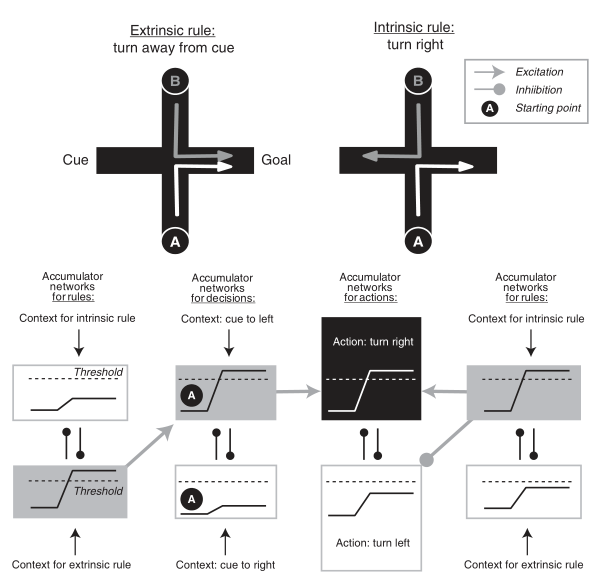
\includegraphics{image_pfc/Fig_3_6}
	\caption*{图3.6基于外在规则与内在规则的选择的累加器网络模型。顶部:大鼠在加号迷宫的A点或B点开始每次试验。对于外在规则,他们需要选择一个与视觉线索相对的目标,在这个例子中是东方。对于内在规则,老鼠需要在选择点右转。底部:累加器网络如何导致两个规则(灰色背景)的右转(黑色背景)的概念描述。例如,当编码外在规则(左下角)的累加器网络达到阈值时,它们的输出抑制编码内在规则(左上角)的网络,并促进编码提示向左的感觉证据的网络,假设大鼠在A点开始试验。这些网络反过来为在这种情况下编码右转的网络提供证据。相反,对于内在规则,不同的网络(右上角)首先达到阈值,并促进右转,同时抑制左转。关键字:带圆圈的字母表示可能的起点。}
\end{figure}
Ragozzino等人(1999年)的一项实验使用了带有气味线索的加号迷宫。在训练老鼠使用一条规则后,Ragozzino等人训练它们使用另一条规则。这种新的学习涉及抑制或超越已经成为习惯的规则。边缘前皮质和边缘下皮质的失活并没有损害大鼠学习初始规则的能力,无论是先学习的规则。但病变确实削弱了转换到第二条规则的能力。确认所涉及的关键因素在两种规则之间切换,而不是一般的切换反应,Ragozzino(2007)测试了大鼠在两种气味的选择之间的切换,大鼠表现正常\par
Rich和Shapiro(2007)使用视觉迷宫外线索扩展了这些结果。边缘前皮质和边缘下皮质的失活导致内在规则和外在规则之间的切换受损,但不会影响大鼠在这两种规则中逆转其选择的能力。重要的是,在规则切换当天,失活并没有影响性能。相反,在第二天进行的测试中,病变导致了旧规则的使用增加和不正确。\par
Rich和Shapiro(2009)还记录了规则转换过程中边缘前和边缘下皮层的神经元活动。他们发现,边缘前皮质的活动变化发生得比边缘下皮质早。当觅食选择在规则改变后有所改善时,边缘下皮层的活动就会发生变化。这一发现可能反映了边缘前皮层提供的对结果导向行为的偏见,而边缘下皮层提供的是对习惯行为的偏见。一般来说,这些区域中的细胞编码内在规则和外在规则之间的切换,但不编码规则内的切换。\par
这些结果表明,边缘前和边缘下皮层在指导基于竞争坐标系的觅食规则的变化。当大鼠试图学习第二条规则时,它们必须使用结果导向的行为来做到这一点,并且它们需要它们的前大脑皮层来产生适当的偏见。如果没有这种偏见,第一条规则中的习惯会干扰第二条规则的学习。如果这第二条觅食规则在很长一段时间内保持有效,老鼠最终会将这条规则作为一种新的习惯。图3.6显示了累加器网络如何实现这些规则,第6-8章更详细地介绍了PF皮层在学习和应用规则中的作用。\par
到目前为止,讨论的重点是内侧PF皮层的边缘前和边缘下部分。下一节研究其剩余的无核成分,即前扣带皮层的作用。\par

\section{利益与成本之间的竞争}
当面临两种行动之间的选择时,动物不仅必须考虑到它们的相对利益,还必须考虑它们的相对成本。在实验室里,实验者可以让动物在以大成本获得的大奖励和以小成本获得的小奖励之间做出选择。作为成本的一个例子,实验者可以要求老鼠爬过障碍物以获得奖励(Salamone等人,1997年),或者在获得奖励之前等待(Cardinal等人,2001年)。第一种操作带来了能源成本;第二种情况会带来延迟成本。\par
Walton等人(2003)使用这些操作中的第一种对具有内侧PF损伤的大鼠进行了测试。在T型迷宫中,老鼠必须在两只手臂之间做出选择。在一只手臂的末端,老鼠可以获得巨大的奖励,但它们只有爬过一道困难的屏障才能达到;在另一只手臂的末端,他们可以获得少量奖励,而无需付出克服障碍所需的努力。正常大鼠选择了两种奖励中较大的一种,尽管它们必须爬上相当大的障碍才能到达在这些条件下,前扣带皮层选择了较小的奖励(图3.7)。诱导老鼠爬上屏障需要相当大的奖励量的增加(Walton等人,2002年)。\par

\begin{figure}[!htb]
	\centering
	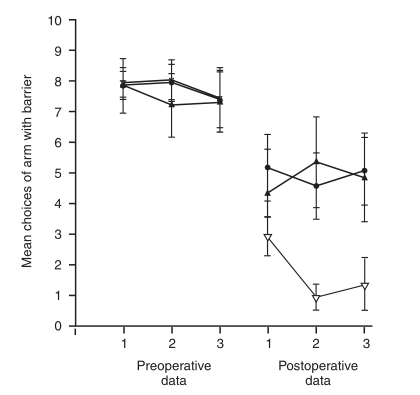
\includegraphics{image_pfc/Fig_3_7}
	\caption*{图3.7努力成本对大鼠目标选择的影响。三组老鼠在迷宫的两臂之间进行选择。一只手臂有少量奖励,没有障碍物;另一只获得了巨大的奖励,并且有一个30厘米高的障碍,老鼠需要克服这个障碍。纵坐标显示了大鼠在10次试验中选择高强度手臂的平均次数。术后,前扣带皮层病变(未填充三角形)的大鼠选择高强度杆的频率明显低于其他两组:假病变(填充圆形)的大白鼠和边缘前加边缘下皮层病变(填充三角形)。误差条:SEM。横坐标上的1、2和3显示了3天的测试数据,每个测试10次。转载自Walton ME、Bannerman DM、Alterescu K、Rushworth MF。前扣带内侧额叶皮层内评估努力相关决策的功能专门化,《神经科学杂志》23:6475-9©神经科学学会,2003年,经许可。}
\end{figure}
Rudebeck等人(2006b)比较了操纵成本在努力或延迟方面的影响。大鼠前扣带皮层的损伤破坏了基于努力的选择,而眶PF皮层的损伤则导致了基于延迟获得奖励的选择受损。因为这项研究涉及大鼠,我们知道病变涉及颗粒缺失区域。在下一章中,我们将研究眼眶PF皮层这些部分的结果,但目前我们可以得出结论,无核PF皮层的内侧部分和眼眶部分都考虑了有关成本和收益的证据,并对所涉及的成本类型进行了一些专门化。我们不知道同样的结论是否适用于猴子,但我们认为它们适用。\par
当一种行为不涉及觅食选择时,前扣带损伤不会损害依赖于努力成本的行为。需要Schweimer和Hauber(2005)大鼠越来越频繁地按下酒吧来获取食物,而前扣带回损伤并没有影响这种行为。如果病变只是让大鼠变得懒惰或冷漠,那么当它们需要进行多次压条来生产食物时,它们就会停止压条。Walton等人(2002)和Schweimer和Hauber(2005)的实验不同之处在于,在前一种情况下,大鼠必须在两种动作之间做出选择,但在后一种情况中,它们没有。沃尔顿等人的实验结果表明,当受损大鼠不得不根据预测结果做出觅食选择时,它们高估了努力成本或低估了回报收益。\par
\subsection{总结}
综上所述,我们利用啮齿类动物的证据证明,内侧PF皮层的无核部分的功能如下:\par
1.它们偏向于系统发育上较老的行为控制系统之间的竞争,以加快觅食选择的适应性。\par
2.它们将觅食选择偏向于适合稳定资源环境的习惯,或偏向于适合中等资源波动条件的结果导向行为。\par
3.它们在外在规则和内在规则之间进行导航选择,以指导觅食选择。\par
4.当动物必须根据预测结果的价值(包括努力成本)在行动之间做出选择时,它们在成本效益分析中发挥着至关重要的作用。\par
在这篇选择性综述中,我们强调了一个结果在奖励方面的当前生物学价值。当然,对结果的评估更广泛地涵盖了其他类型的成本,如捕食或其他形式的伤害的威胁,以及其他类型的利益,如社会利益。\par
内侧PF皮层的连接决定了它如何执行这些功能。
投射到海马体、杏仁核、基底神经节和下丘脑和中脑导水管周围灰质的自主神经控制核可能传达了其自上而下的偏向。来自海马体的输入提供了关于外在坐标系中导航的信息,而来自杏仁核的输入则提供了关于预测结果的当前值的信息。\par

\section{灵长类动物的无核皮层}
在上一节中,证据完全来自作为代表性啮齿类动物的老鼠,也许更有争议的是,作为代表性哺乳动物的老鼠。正如第一章和第二章所解释的,大鼠的所有内侧PF皮层都具有颗粒缺失的细胞结构,就像其他哺乳动物一样。在猕猴中,前扣带回皮层(24区)和边缘下皮层(25区)是无核的,而前边缘皮层(32区)的范围从无核到无颗粒(Vogt和Derbyshire,2009年;Mackey和Petrides,2010年)。猴子25区的亚属位置、细胞结构及其连接(Freedman等人,2000年)支持其被指定为大鼠边缘下皮层的同源物,以及类似的证据支持这样一个结论,即啮齿类动物和灵长类动物的前扣带回、边缘下皮层和边缘前皮层是同源的(第2章)。\par
\subsection{动作反转}
一项关键的实验评估了患有内侧PF病变的猴子在动作之间切换的能力(Kennerley等人,2006年)。在动作反转任务中,猴子要在动作中做出选择。首先,他们学会执行一个动作,例如,在整个试验过程中始终如一地举起手柄。之后,他们必须学会执行另一个动作,例如,在整个试验过程中始终如一地转动手柄。接下来是一系列进一步的反转。
对于每一次逆转,猴子都需要改变自己的动作选择,以产生奖励。偶然性一词通常用来指一项行动与其结果之间的关系。在动作反转任务中,猴子对同一个对象(手柄)执行两个不同的动作。因此,没有任何外部线索促使做出适当的选择。
尽管如此,我们注意到猴子在物体上执行动作。\par
Kennerley等人在前扣带皮层(24区)造成损伤,包括头侧扣带运动区(CMAr)。他们发现,扣带沟皮层受损的猴子在这两种动作之间的切换速度比正常猴子慢(图3.8)\par
\begin{figure}[!htb]
	\centering
	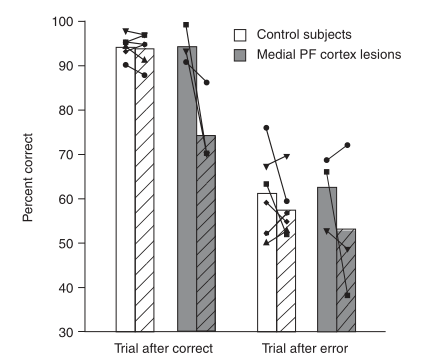
\includegraphics{image_pfc/Fig_3_8}
	\caption*{图3.8行动选择的转回减值。猕猴的术前(实心条)和术后(孵化条)数据。对于正常(对照)猴子(白色)和受损猴子(灰色),正确选择后(左侧四条)和错误选择后(右侧四条)的正确百分比。猴子个体的结果用符号表示,并用线条连接。内侧PF病变涉及前扣带沟的皮层,从沟的吻端到中央前沟的吻顶水平。请注意,受损伤的猴子在正确试验后做出的选择上有更大、更一致的损伤。经麦克米伦出版社有限公司Kennerley SW、Walton ME、Behrens TEJ、Buckley MJ、Matthew F、Rushworth S.的许可转载。最佳决策和前扣带皮层。《自然神经科学》9:940–7,©2006自然出版集团。。}
\end{figure}